%-----------------------------------------
% To process this file:
%   pdflatex fpp-manual
%-----------------------------------------

%\documentclass{article}
\documentclass{hitec}     % Tutorial overall style

\usepackage{index}
\usepackage{xr}
\usepackage{textgreek}
\usepackage{setspace}
\usepackage{graphicx}
\usepackage{moreverb}    % Defines {listing} environment.
\usepackage{amsmath, amsthm, amssymb, amsbsy, mathtools}
\usepackage{alltt}
\usepackage{rotating}
\usepackage{enumitem}
\usepackage{subcaption}
\usepackage{toc-dcs}    % See toc-dcs.sty file in this directory.
\usepackage{xspace}
%%\usepackage{makeidx}
\usepackage[section]{placeins}   % For preventing floats from floating to end of chapter.
\usepackage{longtable}  % For splitting long vertical tables into pieces
\usepackage{multirow}
\usepackage{booktabs}   % For table layouts
\usepackage{yhmath}     % For widehat
\usepackage{xcolor}      % Needed for listings package.
\usepackage{listings}
\usepackage[T1]{fontenc}   % so _, <, and > print correctly in text.
\usepackage[strings]{underscore}    % to use "_" in text
\usepackage[nottoc,numbib]{tocbibind}   % Makes "References" section show in table of contents
\usepackage[pdftex,colorlinks=true,bookmarksnumbered=true]{hyperref}   % Must be last package!

%----------------------------------------------------------------

\newcommand{\sref}[1]{\S\ref{#1}}
\newcommand{\Sref}[1]{Sec.~\sref{#1}}

\newcommand{\vn}{\begingroup\catcode`\_=11 \catcode`\%=11 \dottcmd}
\newcommand\dottcmd[1]{{\usefont{T1}{lmss}{bx}{n} #1}\endgroup}

\newenvironment{example}
  {\vspace{-3.0ex} \begin{alltt}}
  {\end{alltt} \vspace{-2.5ex}}


\definecolor{light-gray}{gray}{0.95}
\lstset{backgroundcolor=\color{light-gray}}
\lstset{xleftmargin=0cm}
\lstset{framexleftmargin=0.3em}

\lstnewenvironment{Xcode}{}{}

\definecolor{lightcyan}{rgb}{0.88, 1.0, 1.0}
\newcounter{main}
\setcounter{main}{1}
\lstnewenvironment{code}[1][firstnumber=\themain,name=main]
  {\lstset{ %language=haskell,
           %columns=fullflexible,
           columns=fixed,
           basicstyle=\small\ttfamily,
           %numbers=left,
           numberstyle=\tiny\color{gray},
           backgroundcolor=\color{lightcyan},
           #1
          }
}
{\setcounter{main}{\value{lstnumber}}}



\definecolor{backcolor}{rgb}{0.8824,1.0,1.0}   % To match code environment
\lstset{basicstyle = \small, backgroundcolor=\color{backcolor}, escapeinside = {@!}{!@}}

\renewcommand{\textfraction}{0.1}
\renewcommand{\topfraction}{1.0}
\renewcommand{\bottomfraction}{1.0}

\settextfraction{0.9}  % Width of text
\setlength{\parindent}{0pt}
\setlength{\parskip}{1ex}
%\setlength{\textwidth}{6in}
\newcommand{\Section}[1]{\section{#1}\vspace*{-1ex}}

\newenvironment{display}
  {\vspace*{-1.5ex} \begin{alltt}}
  {\end{alltt} \vspace*{-1.0ex}}

\title{Fully Polymorphic Package Manual}
%\titlehead{adf}

\author{}
\date{
  \parbox{6in}{
\includegraphics[width=5in]{logo-fpp.pdf}\vspace*{0.4in}} \\ 
  Etienne Forest and David Sagan \\ 
  March 25, 2023
}

\begin{document}

\phantomsection
\pdfbookmark[1]{Cover Page}{Cover Page}
\maketitle

\cleardoublepage
\phantomsection
\pdfbookmark[1]{Contents}{Contents}
\tableofcontents

\newpage

%--------------------------------------------------------------------------------------------------------
\Section{Introduction to FPP/PTC}
\label{s:intro}

FPP/PTC is an object oriented, open source, subroutine library for
\begin{itemize}
\item The manipulation and analysis of Taylor series and Taylor maps.
\item Modeling of charged particle beams in accelerators using Taylor maps.
\end{itemize}
FPP/PTC has two parts. The Fully Polymorphic Package (FPP) is the part that deals with Taylor series and maps. FPP is pure math independent1 of any "physics". The Polymorphic Tracking Code (PTC) part of the library deals with the modeling of particle beams and accelerators. PTC contains the "physics" and relies on FPP for producing and manipulating Taylor maps.
This is illustrated in Figure~\ref{f:ptc}. Roughly, FPP can be subdivided into two parts, a Taylor manipulation part for basic manipulations of Taylor series and an analysis part to do things like normal form analysis. PTC uses the Taylor manipulation part of FPP for things like the construction of Taylor maps. Additionally, PTC uses the analysis tools of FPP. A closer look at FPP shows the existence of a Differential Algebra (DA) package within FPP. This package was originally coded by Martin Berz.

This manual covers the basic usage of FPP and PTC. 

\begin{figure}[tb]
  \centering
  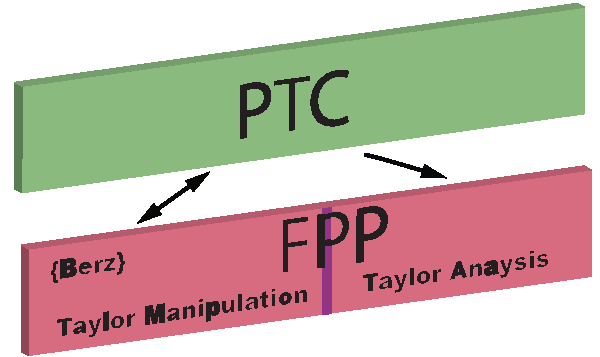
\includegraphics[width=0.8\textwidth]{ptc-fpp.pdf}
  \caption{
The Fully Polymorphic Package (FPP) part of the FPP/PTC library provides manipulation and analysis of Taylor series and maps and the Polymorphic Tracking Code (PTC) part provides the physics from which accelerators can be analyzed.
  }
  \label{f:ptc}
\end{figure}

%--------------------------------------------------------------------------------------------------------
\Section{Where to Obtain FPP/PTC}
\label{s:obtain}

%--------------------------------------------------------------------------------------------------------
\Section{Concepts}
\label{s:concepts}

%-------------------------------------------------------------------
\subsection{Conventions}
\label{s:conventions}

FPP/PTC is written in Fortran90. It is assumed that the reader has some familiarity with this language. In particular, it is assumed that the reader knows what a \vn{structure} is (roughly corresponding to a \vn{class} in Python or C++) which is also called a \vn{derived type}. Also it is assumed that the reader knows about operator overloading.

FPP/PTC uses double precision numbers. The kind type parameter ``\vn{dp}'' is defined in FPP/PTC to correspond to double precision numbers. For example:
\begin{code}
  real(rp) abc, xyz             ! Declare double precision variables abc and xyz.
  xyz = 3.4_dp * abc / 1e9_dp   ! 3.4_dp and 1e9_dp are double precision numbers.
\end{code}

%-------------------------------------------------------------------
\subsection{TPSA Versus DA}
\label{s:tpsa}

TPSA stands for ``Truncated Power Series Algebra'' and DA stands for ``Differential Algebra.'' But what does it mean when applied to a typical accelerator ring? Once we cut the mathematical jargon, we will see that 

\begin{itemize}
\item TPSA operations take into account the constant part and the results change as a function of the order. 
\item DA operations are equivalent to normal TPSA operations used around the closed orbit and thus the constant part of the map is ignored. All the coefficients of the Taylor series stay the same independently of the order invoked. It so happens that the computation of nonlinear differential operators (Lie vector fields for example), are self-consistent because they form a differential algebra. But it is much simpler in our field to state that they are self-consistent because there are no feed down terms.
\end{itemize}

It is important to understand why a non-zero constant part of a Taylor series can be
problematical. To see this, consider TPSA maps of order $N$ from $x$ to $y$ and $y$ to $z$
\begin{align}
  y &= \sum_{j = 0}^N a_j x^j \\
  z &= \sum_{j = 0}^N b_j y^j + \calO(y^{N+1}) \nonumber
\end{align}
In the second equation it is made explicit that since the map is truncated there is an error of
order $N+1$. These maps can be combined to form a TPSA map of $z$ as a function of $x$ 
\begin{equation}
  z = \sum_{j = 0}^N c_j x^j
\end{equation}
If the constant term $a_0$ in the equation from $x$ to $y$ is nonzero, an error term of order higher
than $N$ in the equation from $y$ to $z$ will affect the values of the $c_j$. This is called ``feed
down''. That is, terms of higher order will affect the coefficients of lower order terms when TPSA
maps are combined. To avoid this, maps with zero constant term should be used. With simulations,
this generally means computing maps with respect to the nominal beam orbit. For lattices with a
closed geometry, this generally means computing maps with respect to the closed orbit. For lattices
with an open geometry (EG: Linacs), the reference orbit can be some orbit defined by tracking a beam
from some user-specified initial position.

%-------------------------------------------------------------------
\subsection{Tracking Versus Analysis}
\label{s:tracking.analysis}

An important distiction here is the difference between \vn{tracking} and \vn{analysis}. By
``tracking'' it is meant either the propagation through a lattice of a single particle or a
transport map (which here is always an array of truncated Taylor power series).\footnote
  {
Mathematically, single particle tracking is just tracking of a transport map using Taylor series
truncated at zeroth order. From the code perspective, due to the speed penelely with dealing with
Taylor series, the two are distinct as will be seen in this manual.
  }
This is opposed to ``analysis'' which is the study of a transport map to extract such things as
resonance driving terms, etc. With \vn{fpp}, analysis is always done on maps and not single particle
results. 

As a result of this dicotomy between tracking and analysis, FPP/PTC defines different structures that
are optimized to handle one or the other. Structures that have been designed tohandle tracking are
\begin{example}
  real_8
  complex_8
  probe_8
\end{example}

Why does probe type exist?

%--------------------------------------------------------------------------------------------------------
\Section{Taylor and ComplexTaylor Fundamental Types}
\label{s:fundamental}

FPP defines two fundamental structures that are the building blocks of many other structures:
\vn{Taylor} and \vn{complextaylor}. The \vn{direct} use of either in a tracking program (that is,
when doing simulations with PTC) is discouraged. Rather, other types like \vn{real_8} and \vn{complex_8}
should be used.

%--------------------------------------------------------------------------------------------------------
\subsection{Taylor Type}
\label{s:taylor}

The \vn{taylor} structure overloads the Taylor series of the original real ``DA-Package'' of
Berz. See \sref{sec:real8}. The structure is
\begin{code}
type taylor
   integer i    ! Pointer to Berz
end type taylor
\end{code}
The Berz package uses a positive integer to differentiate different Taylor series and the
\vn{taylor} structure just stores this integer.

%--------------------------------------------------------------------------------------------------------
\subsection{ComplexTaylor Type}
\label{s:taylor}

The \vn{complextaylor} structure stores two Taylor series which represent the real and imaginary parts.
The structure is:
\begin{code}
type complextaylor
   type (taylor) r     ! Real part of complex Taylor series.
   type (taylor) i     ! Imaginary part of complex Taylor series.
end type complextaylor
\end{code}

%--------------------------------------------------------------------------------------------------------
\subsection{Overloaded Operators for Taylor and ComplexTaylor Types}
\label{s:taylor.over}

Overloaded operators for \vn{taylor} and \vn{complextaylor} types include the standard functions
like \vn{sin} and \vn{tanh} as well as the operators used in arithmetic expressions \vn{+}, \vn{-},
\vn{*}, \vn{/}, \vn{**}.

%--------------------------------------------------------------------------------------------------------
\Section{Real_8 Type}
\label{s:real.8}

FPP defines the \vn{taylor} type (\sref{s:taylor} which holds a Taylor series. Since computations
with Taylor series can be slow, FPP defines ``polymorphic'' type called \vn{real_8}.\footnote
  {
The ``8'' here is an allusion to the fact that double precision numbers are generally represented
by 8 bytes and indeed the \vn{dp} parameter defined by PTC/FPP to designate double precision numbers
has, on most systems, a value of 8.
  }
In general, a "polymorphic" variable is a variable that can act in different ways depending on the
context of the code. In this case, a \vn{real_8} variable can act as if it were a real number or it
can act as if it were a Taylor series depending upon how it is initialized. 
An example program will make this clear.
\begin{code}
program real_8_example
use pointer_lattice   ! Read in structure definitions, etc.
implicit none

type (real_8) r8      ! Define a real_8 variable named r8
real(dp) x            ! Define a double precision number

!

nice_taylor_print = .true.    ! Nicely formatted "call print" output
call init (only_2d0, 3, 0)    ! Initialize: #Vars = 2, Order = 3

call alloc(r8)          ! Initialize memory for r8

x = 0.1d0
r8 = x                  ! Initializing r8 to a real will make r8 act as a real.
print "(/,a)", "r8 is now acting as a real:"
call print (r8)         ! Will print a real number.

r8 = 0.7d0 + dz_8(1) + 2*dz_8(2)**3   ! Init r8 as a Taylor series
print "(/,a)", "r8 is now acting as a Taylor series:"
call print(r8)                        ! Will print a Taylor series.

r8 = r8**4  ! Raise the Taylor series to the 4th power
print "(/,a)", "This is r8^4:"
call print (r8)

call kill(r8)
end program
\end{code}
The variable \vn{x} is defined as a double precision real number. The line
\begin{example}
  type (real_8) r8
\end{example}
defines \vn{r8} as an instance of a \vn{real_8} variable and the line
\begin{example}
  call alloc(r8)
\end{example}
initializes \vn{r8}. This initialization must be done before \vn{r8} is used. After \vn{r8} is used,
any memory that has been allocated for use with \vn{r8} is reclaimed by calling the \vn{kill}
routine
\begin{example}
  call kill(r8)
\end{example}
Strictly speaking, \vn{kill} is not necessary here since memory cleanup is automatically done at end
of the program. However, in a subroutine or function, all local instances of \vn{real_8} variables
must be killed otherwise there will be a memory leak.

When \vn{r8} is set to the real number \vn{x} in the line
\begin{example}
    r8 = x
\end{example}
Here the equal sign is overloaded. This initialization of \vn{r8}
will cause \vn{r8} to act as a real number. This is verified by printing the value of \vn{r8} in the lines
\begin{example}
  print '(/,a)', "r8 is now acting as a real:"
  call print (r8)
\end{example}
The output is just a single real number indicating that \vn{r8} is acting as a real:
\begin{example}
  r8 is now acting as a real:"
  0.100000000000000
\end{example}
Notice that the \vn{print} statement uses the Fortran intrinsic print function while the \vn{call
print} statement uses the overloaded print subroutine defined by \vn{FPP}.

When \vn{r8} is set to a Taylor series in the line
\begin{example}
  r8 = 0.7d0 + dz_8(1) + 2*dz_8(2)**3 ! Init r8 as a Taylor series
\end{example}
this will cause \vn{r8} to act as a Taylor series. To understand how this initialization works,
first consider the initialization of FPP/PTC which was done by the line
\begin{example}
  call init (only_2d0, 3, 0)  ! Initialize FPP/PTC. #Vars = 2, Order = 3
\end{example}
The first argument, \vn{only_2d0}, is a parameter defined by \vn{PTC}.\footnote
  {
The \vn{only_2d0} parameter is of type \vn{internal_state} (\sref{s:internal}). When an
\vn{internal_state} type is used as the first argument in the overloaded routine \vn{init}, both
\vn{FPP} and \vn{PTC} will be initialized.
  }
When \vn{only_2d0} is used as the first argument to \vn{init}, the number of variables will be two
which is appropriate for simulations involving motion along one axis (typically involving phase
space $(x, p_x)$).\footnote
  {
There is also an \vn{only_4d0} parameter for configuring using 4 variables for simulations with
transverse phase space $(x, p_x, y, p_y)$. However, there is no \vn{only_6d0} parameter sice
configuring for the full 6D phase space is a bit more complicated (involving consideration like
whether there are powered RF cavities or not).
  }
If only \vn{FPP} needs to be initialized (as is the case at hand), the initialization here could
have been done in the above example via:
\begin{example}
  call init (3, 2)  ! Initialize just FPP. Order = 3, #Vars = 2 (Notice reversed order!)
\end{example}
The second argument, \vn{3}, gives the order at which the Taylor series is truncated to. That is, after this initialization, all Taylor series $t$ will be of the form:
\begin{equation}
    t = \sum_{i,j}^{0 \le i+j \le 3} C_{ij} \, z_1^i \, z_2^j
\end{equation}
where $z_1$ is the first variable and $z_2$ is the second variable.  \vn{FPP} sets up an array named
\vn{dz_8} such that \vn{dz_8(N)} represents the $N$\Th variable. Thus in the above code
\vn{r8} is initialized to the Taylor series:
\begin{equation}
    t = 0.7 + z_1 + 2 \, z_2^3
\end{equation}
This is confirmed by printing \vn{r8} after it has been set via the lines
\begin{example}
  print '(/,a)', "r8 is now acting as a Taylor series:"
  call print(r8)
\end{example}
The output is:
\begin{example}
r8 is now acting as a Taylor series:
Out  Order  Coef                     Exponents
-----------------------------------------------------------
  1:     0  0.7000000000000000       0  0
  1:     1   1.000000000000000       1  0
  1:     3   2.000000000000000       0  3
\end{example}
Each line in the above output, after the line with dashes, represents one term in the Taylor
series. The general form for printing a Taylor term is:
\begin{example}
  <output-index> <term-order>   <term-coefficient>    <z1-exponent>  <z2-exponent>, ...
\end{example}
The \vn{<output-index>} is the index of the output variable. Here, since there is only one Taylor
series and not an array, that index is one.  The \vn{<term-order>} is the order of the term. That is, the
sum of the exponents. For example, the last line in the above printout is
\begin{example}
  1:     3   2.000000000000000       0  3
\end{example}
This line represents the term $2 \, z_1^0 \, z_2^3$ which is order 3. 

Once \vn{r8} has been initialized, it can be used in expressions. Thus the line
\begin{example}
  r8 = r8**4  ! Raise the Taylor series to the 4th power
\end{example}
raises \vn{r8} to the 4th power and puts the result back into \vn{r8}. This is confirmed by the
final print which produces
\begin{example}
This is r8^4:
Out  Order  Coef                     Exponents
-----------------------------------------------------------
  1:     0  0.2400999999999999       0  0
  1:     1   1.372000000000000       1  0
  1:     2   2.940000000000000       2  0
  1:     3   2.800000000000000       3  0
  1:     3   2.743999999999999       0  3
\end{example}
Notice that the map has been truncated so that no term has an order higher than 3 as
expected. Expressions using \vn{real_8} variables involve overloaded operators as discussed in
section \sref{s:over}.

%--------------------------------------------------------------
\subsection{Real\_8 Under the Hood}\label{sec:real8}

The particulars of how the \vn{real_8} structure is defined are generally not of interest to the
general user. But it is instructive to take a quick look. In the \vn{FPP} code the \vn{real_8}
structure is defined as:
\begin{example}
type real_8
   type (taylor) t   ! Used if taylor
   real(dp) r        ! Used if real
   integer kind      ! 0,1,2,3 (1=real,2=taylor,3=taylor knob)
   integer i         ! Used for knobs and special kind=0
   real(dp) s        ! Scaling for knobs and special kind=0
   logical(lp) :: alloc  ! True if taylor is allocated in da-package
end type real_8
\end{example}
The \vn{t} component of the structure is of type \vn{taylor} (\sref{s:taylor}) and is used if a
\vn{real_8} variable is acting as a Taylor series. The \vn{r} component is used if a \vn{real_8}
variable is acting as a real number. The \vn{kind} component is an integer that sets the behavior of
a \vn{real_8} variable. Besides behaving as \vn{real} or a Taylor series, a \vn{real_8} variable may
behave as a "\vn{knob}" which will be explained later.  The reason for hiding a Taylor series under
the hood is to defer the decision of its use to run time.

This is useful when
tracking since manipulating Taylor series is computationally more expensive than using real numbers.

%-------------------------------------------------------------------
\Section{Complex\_8 Type}
\label{s:c8}

The type \vn{complex_8} is the polymorphic version of the \vn{complextaylor} type just as the
\vn{real_8} type is the polymorphic version of the \vn{taylor} type.

The type \vn{complex_8} is rarely used in a tracking code since all quantities we compute are
ultimately real. However once in a while it is useful to go into complex coordinates temporarily. If
the type \vn{complex_8} did not exist, then a code could become extremely difficult to write. This
happens a lot when Maxwell's equations are written in cylindrical coordinates. In such a case, if
${\bf z}=(x,p_x,y,p_y)$, then most intermediate calculations involve a quantity $q=x+i\,y$. It in
such a case, the complex polymorph is useful. This happens in the tracking code for some magnets in
PTC but it is generally hidden from a normal programmer using PTC.

The definition of \vn{complextaylor} is: 
\begin{example}
type complex_8
  type (complextaylor) t 
  complex(dp) r
  logical(lp) alloc
  integer kind
  integer i,j 
  complex(dp) s
end type complex_8
\end{example}
As in the case of the real polymorph, the \vn{t} component contains the complex Taylor series and
the \vn{r} component contains the complex number if the polymorph is not a Taylor series.

%-------------------------------------------------------------------
\Section{Real_8 and Complex_8 Functions and Operators}
\label{s:real.op}

Operators that act on \vn{real_8} and \vn{complex_8} types:
\begin{example}
  exp(t)          ! Exponentiation
  log(t)          ! Log
  sin(t), sind(t) ! Sine radians and deg
  cos(t), cosd(t)
  tan(t), tand(t)
  acos(t)
  asin(t)
  atan(t), atand(t)
  atan2(ty, tx), atan2d(ty, tx)
  sinx_x(t)
  sinhx_x(t)
  abs(t) 
  full_abs(t)???? What is this
  dble ???? is this the same as real?
  real(ct), aimag(ct)
  cmplx(t_re, t_im)
\end{example}

Question: Do all functions act on real_8, taylor, complex_8, complextaylor?


%-------------------------------------------------------------------
\Section{Internal_State Type}
\label{s:internal}

Components of the \vn{internal_state} structure define parameters that affect such things as whether RF cavities are considered to be on or off or how phase space variables are treated. The structure definition is:
\begin{example}
type internal_state
   integer totalpath      ! T => total time or path length is used
   logical(lp) time       ! T => Time is used instead of path length
   logical(lp) radiation  ! T => Radiation is turned on
   logical(lp) nocavity   ! T => Cavity is turned into a drift
   logical(lp) fringe     ! T => Fringe fields are turned on (mainly for quadrupoles)
   logical(lp) stochastic ! T => Random Stochastic kicks to x(5)
   logical(lp) envelope   ! T => Stochastic envelope terms tracked in probe_8
   logical(lp) para_in    ! T => Parameters in the map are included
   logical(lp) only_4d    ! T => Real_8 Taylor in (x,p_x,y,p_y)
   logical(lp) delta      ! T => Real_8 Taylor in (x,p_x,y,p_y,delta)
   logical(lp) spin       ! T => spin is tracked
   logical(lp) modulation ! T => One modulated family tracked by probe
   logical(lp) only_2d    ! T => Real_8 taylor in (x,p_x)
   logical(lp) full_way   !
end type internal_state

For each structure component except \vn{param_in} and \vn{full_way}, there is a global parameter defined 




%-------------------------------------------------------------------
\Section{Knobs}
\label{sec:real8code}

This type is the most important type if you write a tracking code of respectable length.  Imagine that your code tracks in one degree of freedom (1-d-f). Then you will push two phase space variables through your magnets, let us call them ${\bf z}=(z_1,z_2)$. These variables will denote  the position and the tangent of an angle in our little example.  If it is your  intention to always extract a Taylor series around a special orbit, then  it would suffice to declare as \vn{taylor} only the phase space variables ${\bf z}=(z_1,z_2)$ and any temporary variables the code might used during its calculations. 

But what if we want to have a Taylor map that also depends upon some parameter or parameters of the lattice. For example, a map can include quadrupole strengths as independent variables in the maps. Such variables are called ``\vn{knobs}.'' Since this is a user decision, it is best if the code decides at execution time using the type \vn{real_8}.
As an example, consider the code \vn{z_why_polymorphism.f90}:

\begin{code}
program my_small_code_real_8
use polymorphic_complextaylor
implicit none
type(real_8) :: z(2)  
real(dp) :: z0(2) = [0, 0]  ! special orbit
type(reaL_8)  :: L , B, K_q , K_s 
integer :: nd = 1 , no = 2 , np = 0, ip
longprint = .false.         ! Shorten "call print" output
! nd = number of degrees of freedom
! no =  order of Taylor series
! Number of extra variables beyond 2*nd

call alloc(z)
call alloc( L , B, K_q , K_s )
np=0
print * , "Give  L and parameter ordinality (0 if not a parameter)"
read(5,*) L%r , ip
np=np+ip
call make_it_knob(L,ip);  np=np+ip;
print * , "Give  B  and parameter ordinality (0 if not a parameter)"
read(5,*) K_q%r , ip
print * , "Give  K_q and parameter ordinality (0 if not a parameter)"
read(5,*) K_q%r , ip
call make_it_knob(K_q,ip);  np=np+ip;
print * , "Give  K_s and parameter ordinality (0 if not a parameter)"
read(5,*) K_s%r , ip
call make_it_knob(K_s,ip); np=np+ip;
print * , "The order of the Taylor series ?"
read(5,*) no

call init(no,nd,np) ! Initializes TPSA 

z(1)=z0(1) + dz_8(1) ! <--- Taylor monomial z_1 added
z(2)=z0(2) + dz_8(2) ! <--- Taylor monomial z_2 added

call track(z)

call print(z)

contains

subroutine track(z)
implicit none
type(real_8) :: z(2) 
 z(1)=z(1)+L*z(2) 
 z(2)=z(2)-B-K_q*z(1)-K_s*z(1)**2 
end subroutine track

end program my_small_code_real_8
\end{code}

In this little code, there is one drift of length \vn{L} followed by a multipole kick that contains a dipole of strength \vn{B}, a quadrupole of strength \vn{K_q} and a sextupole of strength \vn{K_s}. We run the code ignoring the parameters:

\begin{example}
 Give  L and parameter ordinality (0 if not a parameter)
1 0
 Give  B  and parameter ordinality (0 if not a parameter)
0 0
 Give  K_q and parameter ordinality (0 if not a parameter)
.1 0
 Give  K_s and parameter ordinality (0 if not a parameter)
0 0
 The order of the Taylor series ?
2

 Properties, NO =    2, NV =    2, INA =   20
 *********************************************

   1   1.000000000000000       1  0
   1   1.000000000000000       0  1


 Properties, NO =    2, NV =    2, INA =   21
 *********************************************

   1 -0.1000000000000000       1  0
   1  0.9000000000000000       0  1
\end{example}

This little program produces Taylor series to second order in the phase space variables ${\bf z}=(z_1,z_2)$ similar to the programs \vn{Transport} and \vn{Marylie}.
However, we can now require that the multipole strengths be variables of the Taylor series without recompiling the program. In this example, we make the quadrupole strength the third variable of TPSA:  $K_q=0.1 + dz_3$.

\begin{example}
 Give  L and parameter ordinality (0 if not a parameter)
1 0
 Give  B  and parameter ordinality (0 if not a parameter)
0 0
 Give  K_q and parameter ordinality (0 if not a parameter)
.1 1
 Give  K_s and parameter ordinality (0 if not a parameter)
0 0
 The order of the Taylor series ?
2

 Properties, NO =    2, NV =    3, INA =   22
 *********************************************

   1   1.000000000000000       1  0  0
   1   1.000000000000000       0  1  0


 Properties, NO =    2, NV =    3, INA =   23
 *********************************************

   1 -0.1000000000000000       1  0  0
   1  0.9000000000000000       0  1  0
   2  -1.000000000000000       1  0  1
   2  -1.000000000000000       0  1  1
\end{example}

Again, we must emphasize that while it would have been easy here to use the type \vn{taylor} for all the variables, it is totally unfeasible in a real tracking code to either recompile the code or allow all parameters of the systems to be Taylor series. This is why typical matrix\footnote{This is not true of Berz's COSY INFINITY which handles variable memory of TPSA within its own internal language.} codes, not using TPSA, are limited to a small set of Taylor variables, usually the six phase space variables.

So in summary a \vn{real_8} polymorph can be as mentioned in \sref{s:real8}:

\begin{enumerate}
 \item A real number
 \item a Taylor series with real coefficients (\vn{taylor})
 \item a knob which is a simple temporary Taylor series activated only if needed
\end{enumerate}

%-------------------------------------------------------------------
\Section{Manual To Do List}


Note: calling init again wipes out existing Taylor series. (Does is wipe out universial taylor?)

Explain knobs

\end{document}


